\subsection{Saddle Points}
\label{sec:sps}

Saddle points are stationary points, i.e. with zero gradient, on a multidimensional function, $f(\vR)$, that are neither maxima nor minima.

\begin{figure}
  \begin{center}
    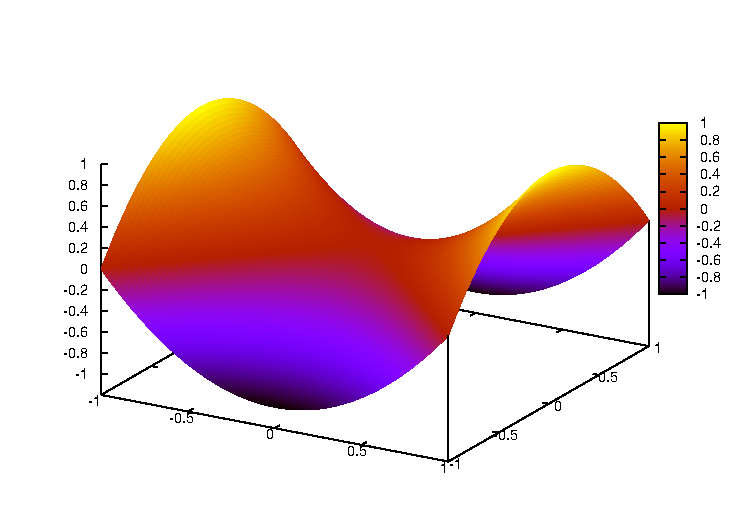
\includegraphics[width=0.6\linewidth]{saddle-point}
    \parbox{0.85\linewidth}{
      \caption{A first order saddle point.
      $f(x=0, y=0) = x^2 - y^2$. A minimum in the $x$ direction and a maximum in the $y$ direction.
      }}
    \label{fig:saddle-point}
  \end{center}
\end{figure}

A common view of a saddle (point) is the function $f(x, y) = x^2 - y^2$ which near $(x,y) = (0,0)$ resembles a saddle, used when riding horses (see \fref{fig:saddle-point}), curving upwards in one direction and downwards in the other.
\figmiss{Comparison of a saddle points environment and a saddle used on a horse.}
This most common image of a saddle point lacks a few elements to be to tell their whole story.
On functions of higher dimensionality than $2$, different orders of saddle points are possible.
The order of the saddle point is decided by the amount of directions that are at a maximum, rather than a minimum, or the non-positive eigenvalues of the Hessian.
As such, figure ... show a first order saddle point on a two dimensional function.

The Hessian at the saddle point displayed in \fref{fig:saddle-point} has one negative eigenvalue, however, a saddle point with a zero eigenvalue is also possible, such as the 1D example $f(x = 0) = x^3$. \figmiss{1D saddle point}

Locating saddle points in multiple dimensions is a non-trivial task as only a limited number of steepest decent paths lead to each one while the majority lead to minima.
A number of schemes have been suggested ...

\recent

\incomplete
